\documentclass[a4j]{jarticle}

%% "%:"から始まる行を書くと「タグ行」として扱われる。Command+2でタグ行を挿入

\usepackage{url}
\usepackage{graphicx}
\usepackage{ascmac}
\usepackage{here}
\usepackage{itembkbx}

\newenvironment{ite}{\begin{itemize}}{\end{itemize}} %箇条書き
\newenvironment{tab}{\begin{table}}{\end{table}} %表
\newenvironment{cen}{\begin{center}}{\end{center}} %中央揃え
\newenvironment{tabu}{\begin{tabular}}{\end{tabular}} %表
\newenvironment{bbox}{\begin{breakbox}}{\end{breakbox}} %四角囲い付け
\newenvironment{scr}{\begin{breakscreen}}{\end{breakscreen}} %丸囲い付け
\newenvironment{bit}{\begin{breakitembox}}{\end{breakitembox}} %囲い付き箇条書き, [c]等必要, {}に題名
\newenvironment{fig}{\begin{figure}}{\end{figure}} %図
\newenvironment{enu}{\begin{enumerate}}{\end{enumerate}} %箇条書き(数字)
\newenvironment{des}{\begin{description}}{\end{description}} %箇条書き(文字)
\newcommand{\ma}{main関数}
\newcommand{\mo}{move関数}
\newcommand{\pa}{path\_print関数}
\newcommand{\pai}{paint関数}

% 講義・演習名
\newcommand{\lectureName}{情報科学演習C}
% レポートの回数
\newcommand{\reportNumber}{1}
% レポートのタイトル
\newcommand{\reportTitle}{}
% 教員名
\newcommand{\teacherName}{小島 英春,内山 彰 教員}
% 課題締め切り日
\newcommand{\deadline}{2018年4月23日(月) 12:59}

% 提出者名
\newcommand{\studentName}{川上 遼太}
% 提出者所属
\newcommand{\studentAff}{基礎工学部 情報科学科 計算機科学コース 3年}
% 提出者学籍番号
\newcommand{\studentID}{09B16022}
% 提出者電子メールアドレス
\newcommand{\studentEmail}{u407773h@ecs.osaka-u.ac.jp}
% 課題提出日
\newcommand{\submitted}{2018年4月23日(月)}


\begin{document}

%Title page start
\begin{titlepage}
\mbox{\vspace{10cm}}

\begin{center}
{\Huge\bfseries
\lectureName \\
第\reportNumber{}回レポート} \\
\vspace{1cm}
{\Large \reportTitle}
\vspace{5cm}

{\large
\begin{tabular}{rcl}
担当教員 & : & \teacherName \\
提出者   & : & \studentName \\
所属/学年   & : & \studentAff\\
学籍番号 & : & \studentID \\
電子メール & : & \texttt{\studentEmail}\\
\\
提出日 & : & \submitted \\
締切日 & : & \deadline
\end{tabular}
}
\end{center}
\end{titlepage}
%Title page end

\tableofcontents
\newpage

\section{課題内容}


\section{課題1-1}

\subsection{(1.)}
\label{1-1-1}

以下に
\begin{verbatim}
$ ping exp101
\end{verbatim}
と入力した時の出力結果を記載する.

\begin{bit}[l]{(1.)出力結果}
\small{
\begin{verbatim}
 1 r-kawakm@exp006:~$ ping exp101
 2	PING exp101.exp.ics.es.osaka-u.ac.jp (192.168.16.65) 56(84) bytes of data.
 3	64 bytes from exp101.exp.ics.es.osaka-u.ac.jp (192.168.16.65):
  icmp_seq=1 ttl=64 time=0.159 ms
 4	64 bytes from exp101.exp.ics.es.osaka-u.ac.jp (192.168.16.65):
  icmp_seq=2 ttl=64 time=0.189 ms
 5	64 bytes from exp101.exp.ics.es.osaka-u.ac.jp (192.168.16.65):
  icmp_seq=3 ttl=64 time=0.238 ms
 6	64 bytes from exp101.exp.ics.es.osaka-u.ac.jp (192.168.16.65):
  icmp_seq=4 ttl=64 time=0.168 ms
 7	64 bytes from exp101.exp.ics.es.osaka-u.ac.jp (192.168.16.65):
  icmp_seq=5 ttl=64 time=0.187 ms
 8	64 bytes from exp101.exp.ics.es.osaka-u.ac.jp (192.168.16.65):
  icmp_seq=6 ttl=64 time=0.180 ms
 9	64 bytes from exp101.exp.ics.es.osaka-u.ac.jp (192.168.16.65):
    icmp_seq=7 ttl=64 time=0.194 ms
10	64 bytes from exp101.exp.ics.es.osaka-u.ac.jp (192.168.16.65):
    icmp_seq=8 ttl=64 time=0.232 ms
11	64 bytes from exp101.exp.ics.es.osaka-u.ac.jp (192.168.16.65):
    icmp_seq=9 ttl=64 time=0.167 ms
12	64 bytes from exp101.exp.ics.es.osaka-u.ac.jp (192.168.16.65):
    icmp_seq=10 ttl=64 time=0.193 ms
13	^C
14	--- exp101.exp.ics.es.osaka-u.ac.jp ping statistics ---
15	10 packets transmitted, 10 received, 0% packet loss, time 8999ms
16	rtt min/avg/max/mdev = 0.159/0.190/0.238/0.029 ms
\end{verbatim}
}
\end{bit}

2行目ではFQDNである"exp101.exp.ics.es.osaka-u.ac.jp"のIPアドレスが192.168.16.65であることがわかった.

3-12行目ではほとんど同じことが記述されているため3行目を例に挙げて説明する.

\begin{verbatim}
64 bytes from exp101.exp.ics.es.osaka-u.ac.jp (192.168.16.65):
icmp_seq=1 ttl=64 time=0.159 ms
\end{verbatim}

"64 bytes from exp101.exp.ics.es.osaka-u.ac.jp (192.168.16.65)"は接続確認先であるexp101.exp.
ics.es.osaka-u.ac.jp (192.168.16.65)に導通試験を行うのに送信したデータのバイト数であり,これが64byteであるということである.また,"icmp\_seq=1"では簡単に言えば,何回目の導通試験を行っているかを表している.ただし,正しくはicmpパケットデータの何番目のデータ送信かという意味である."ttl=64"はttlのあたいはホストのOSで決められた初期値から,経由したルーターの数を引いたものである.Windowsの初期値は128,Linuxは64,Solarisは255である.今回はttl=64であるからホストのOSはLinuxであることがわかる."time=0.159 ms"は簡単に言えば通信速度であり,詳しくはpingコマンドを実行した計算機が導通試験のパケットデータを発してから相手先からのリアクションが戻ってくるまでの時間であり,今回は0.159ms秒である.

15行目では10回の導通試験を行ったということであり,失敗したパケットはないということである
.このtimeはpingコマンドを始めてから終了するまでの時間である.

16行目のrttは通信速度の基本統計量データである.min(最速値)/max(最遅値)/ave(平均値)
/mdev(通信速度の偏差)の順に行ったパケット通信の結果を出力している.

\subsection{(2.)}

\begin{figure}[htb]
\centering
\includegraphics[width=.65\textwidth]{w-higashi.eps}
\caption{"\url{http://www-higashi.ist.osaka-u.ac.jp/}"での検索結果}
\label{fig:www}
\end{figure}

\begin{figure}[htb]
\centering
\includegraphics[width=.65\textwidth]{133-higashi.eps}
\caption{"\url{http://133.1.17.66/}"での検索結果}
\label{fig:133}
\end{figure}

図\ref{fig:www}と図\ref{fig:133}からわかるように"\url{http://www-higashi.ist.osaka-u.ac.jp/}"と"\url{http://133.1.17.66/}"は同じホームページを指している.

\begin{tab}[H]
\centering
\begin{tabu}{|c|c|}
\hline
ドメイン名 & \url{www-higashi.ist.osaka-u.ac.jp} \\
\hline
IPアドレス & 133.1.17.66 \\
\hline
\end{tabu}
\caption{ドメイン名とIPアドレス}
\label{tab:ip}
\end{tab}

ドメイン名は英数字からなっているため人が見てもわかりやすくなっているのに対し,IPアドレスは数字だけからなっていて人が見てもなかなか理解できない.しかし,数字だけからなっているということは機械には理解しやすいということである.ここでDNS(Domain Name System)と言うシステムを紹介しよう.DNSとは人にとって理解しやすいドメイン名を機会が理解しやすいIPアドレスに対応づける仕組みである.このDNSがあるために表\ref{tab:ip}のドメイン名とIPアドレスは同じものとみなすことができ,"\url{http://www-higashi.ist.osaka-u.ac.jp/}"と"\url{http://133.1.17.66/}"は同じホームページが開かられようになっている.

\subsection{(3.)}

%% 1と2の結果にもnslookupコマンドを実行してみて,考察する.
%% 画像も貼り付ける.

nslookupコマンドとはDNSサーバーから対象となるドメイン名またはIPアドレスに対応するIPアドレスまたはドメイン名を返すコマンドであり,以下に(1.)と(2.)の"exp004"(この時点ではexp004が割り当てられていたためexp101ではない)と"\url{www-higashi.ist.osaka-u.ac.jp}"に対してnslookupコマンドを実行した時の出力結果を記載する.

\begin{bit}[l]{(1.)と(2.)に対してのnslookupコマンドの出力結果}
\small{
\begin{verbatim}
 1	r-kawakm@exp004:~$ nslookup exp004
 2	Server:		192.168.25.6
 3	Address:	192.168.25.6
 4
 5	Name:	exp004.exp.ics.es.osaka-u.ac.jp
 6	Address: 192.168.16.17
 7
 8	r-kawakm@exp004:~$ nslookup www-higashi.ist.osaka-u.ac.jp
 9	Server:		192.168.25.6
10	Address:	192.168.25.6#53
11
12	Non-authoritative answer:
13	Name:	www-higashi.ist.osaka-u.ac.jp
14	Address: 133.1.17.66
\end{verbatim}
}
\end{bit}

nslookupコマンドの実行結果ではまずDNSサーバーのIPアドレスがわかり,その後目的とするドメイン名またはIPアドレスがわかるのが成功した時である.実際にexp004を引数としてnslookupコマンドを実行してみた時の実行結果は1-7行である.この例では"192.168.25.6"が接続したDNSサーバーであり,exp004の省略なしのドメイン名は"\url{exp004.exp.ics.es.osaka-u.ac.jp}"であり,対応するIPアドレスが"192.168.16.17"であることがわかった.次に8-14行は"\url{www-higashi.ist.osaka-u.ac.jp}"を引数としてnslookupコマンドを実行した時の結果である."exp004"の時と異なるのは12行目である"Non-authoritative answer:"と言う文言である.これは信頼できる筋の情報ではないということであり,過去にDNSサーバー"192.168.25.6"が過去にドメイン名"\url{www-higashi.ist.osaka-u.ac.jp}"に対応するIPアドレス"133.1.17.66"にアクセスしたことがあり,その結果を一定時間DNSキャッシュに保存していたために実際に探索をせずにキャッシュデータを出力したと言うために信頼できないされているのである.

\\

次に"\url{http://www-ise4.ist.osaka-u.ac.jp}"に対応するIPアドレスをnslookupコマンドを用いて調べてみる.

\begin{bit}[l]{(3.)出力結果}
\small{
\begin{verbatim}
1	r-kawakm@exp072:~$ nslookup www-ise4.ist.osaka-u.ac.jp
2	Server:		192.168.25.6
3	Address:	192.168.25.6#53
4
5	Non-authoritative answer:
6	Name:	www-ise4.ist.osaka-u.ac.jp
7	Address: 133.1.16.2
\end{verbatim}
}
\end{bit}

上記の出力結果からわかるように"\url{http://www-ise4.ist.osaka-u.ac.jp}"に対応するIPアドレスは"\url{http://133.1.16.2/}"であることがわかった.実際にブラウザでURLを入力して検索してみたところ下図\ref{fig:w-ise}と図\ref{fig:133-ise}のようになり,(2.)と同じように同じホームページにアクセスされることがわかり,nslookupコマンドでわかったドメイン名とIPアドレスがDNSで対応していることがわかった.

\begin{figure}[htb]
\centering
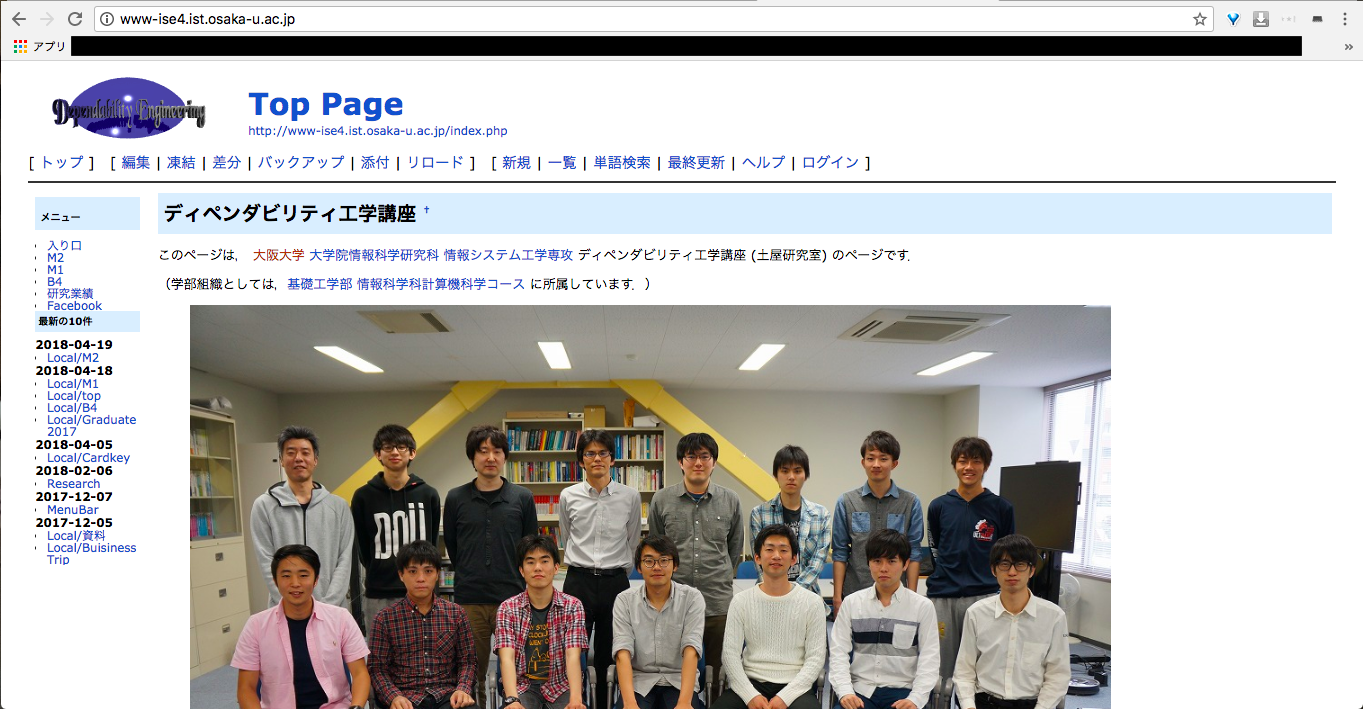
\includegraphics[width=.65\textwidth]{w-ise.eps}
\caption{"\url{http://www-ise4.ist.osaka-u.ac.jp}"での検索結果}
\label{fig:w-ise}
\end{figure}

\begin{figure}[htb]
\centering
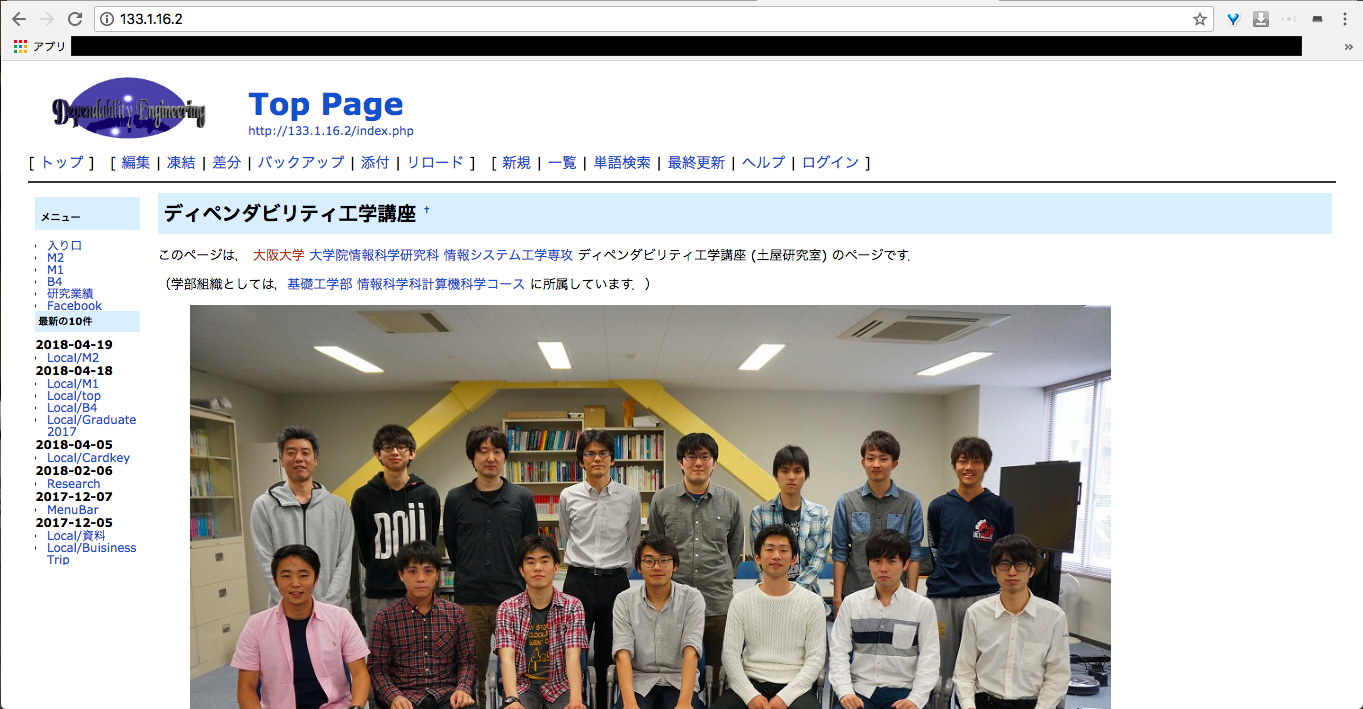
\includegraphics[width=.65\textwidth]{133-ise.eps}
\caption{"\url{http://133.1.16.2/}"での検索結果}
\label{fig:133-ise}
\end{figure}

\section{課題1-2}


\subsection{(4.)}
\label{1-1-4}

以下に
\begin{verbatim}
$ /usr/sbin/arp -a
\end{verbatim}
と入力した時の出力結果を記載する.

\begin{bit}[l]{(4.)出力結果}
\small{
\begin{verbatim}
1	r-kawakm@exp072:~$ /usr/sbin/arp -a
2	svm-01.exp.ics.es.osaka-u.ac.jp (192.168.16.241) at 02:a0:98:c4:b2:cf
  [ether] on ens192
3	? (192.168.16.254) at 14:18:77:10:31:aa [ether] on ens192
4	exp017.exp.ics.es.osaka-u.ac.jp (192.168.16.4) at 00:50:56:b7:7b:db
  [ether] on ens192
5	dhcp-01.exp.ics.es.osaka-u.ac.jp (192.168.16.240) at 00:50:56:b7:21:6e
  [ether] on ens192
6	cups.exp.ics.es.osaka-u.ac.jp (192.168.16.253) at 00:50:56:b7:5b:4b
  [ether] on ens192
\end{verbatim}
}
\end{bit}

arpコマンドは,ARP(Address Resolution Protocol)テーブルの表示/設定を行うコマンドである.そもそもARPテーブルとは,イーサネット通信のために用いられるIPアドレスとMACアドレスの対照表である.ここで必要なIPアドレスは最終目的地となる端末のIPアドレスであり,MACアドレスとは次に通る端末の住所のようなものである.そのため,MACアドレスは端末を通るたびに更新される.目的地のIPアドレスがわかっていてもMACアドレスがわかっていないため,arpコマンドによって他の端末に自身のIPアドレスとMACアドレスとさらに目的地のIPアドレスをブロードキャストして,関係のある端末にその信号が届いたらユニキャストで元の端末にその端末のIPアドレスとMACアドレスを送信する.この送信された情報をarpテーブルで記憶しておく.

今回の出力結果は5組のIPアドレスとMACアドレスとそのARPテーブルを管理しているインターフェイスが表示されている.この内容はarpテーブルに保存される時間内に通信した端末のIPアドレスとMACアドレスであり,もう一度この中のいづれかを経由したり,到達地とした時にはこのarpテーブルの情報が使われる.

2-6行目の出力は出力されている内容は対象が違うだけでコマンドの出力としては違いがないため2行目を例にあげて説明する.

\begin{tab}[H]
\centering
\begin{tabu}{|c|c|}
\hline
ホスト名 & \url{svm-01.exp.ics.es.osaka-u.ac.jp} \\
\hline
IPアドレス & 192.168.16.241 \\
\hline
Macアドレス & 02:a0:98:c4:b2:cf \\
\hline
インターフェイス & ens192 \\
\hline
\end{tabu}
\caption{2行目のARPテーブル}
\label{tab:arp}
\end{tab}

\subsection{(5.)}
\label{sec:5.}

以下に
\begin{verbatim}
$ /bin/ping exp101
↓ その後
$ /usr/sbin/arp -a
\end{verbatim}
と入力した時の出力結果を記載する.

\begin{bit}[l]{(5.)出力結果}
\small{
\begin{verbatim}
 1	r-kawakm@exp072:~$ /usr/sbin/arp -a
 2	svm-01.exp.ics.es.osaka-u.ac.jp (192.168.16.241) at 02:a0:98:c4:b2:cf
  [ether] on ens192
 3	? (192.168.16.254) at 14:18:77:10:31:aa [ether] on ens192
 4	exp017.exp.ics.es.osaka-u.ac.jp (192.168.16.4) at 00:50:56:b7:7b:db
  [ether] on ens192
 5	dhcp-01.exp.ics.es.osaka-u.ac.jp (192.168.16.240) at 00:50:56:b7:21:6e
  [ether] on ens192
 6	cups.exp.ics.es.osaka-u.ac.jp (192.168.16.253) at 00:50:56:b7:5b:4b
  [ether] on ens192
 7	r-kawakm@exp072:~$ /bin/ping exp101
 8	PING exp101.exp.ics.es.osaka-u.ac.jp (192.168.16.65) 56(84) bytes of
  data.
 9	64 bytes from exp101.exp.ics.es.osaka-u.ac.jp (192.168.16.65):
  icmp_seq=1 ttl=64 time=0.579 ms
10	64 bytes from exp101.exp.ics.es.osaka-u.ac.jp (192.168.16.65):
    icmp_seq=2 ttl=64 time=0.193 ms
11	64 bytes from exp101.exp.ics.es.osaka-u.ac.jp (192.168.16.65):
    icmp_seq=3 ttl=64 time=0.216 ms
12	64 bytes from exp101.exp.ics.es.osaka-u.ac.jp (192.168.16.65):
    icmp_seq=4 ttl=64 time=0.191 ms
13	64 bytes from exp101.exp.ics.es.osaka-u.ac.jp (192.168.16.65):
    icmp_seq=5 ttl=64 time=0.205 ms
14	64 bytes from exp101.exp.ics.es.osaka-u.ac.jp (192.168.16.65):
    icmp_seq=6 ttl=64 time=0.210 ms
15	64 bytes from exp101.exp.ics.es.osaka-u.ac.jp (192.168.16.65):
    icmp_seq=7 ttl=64 time=0.237 ms
16	64 bytes from exp101.exp.ics.es.osaka-u.ac.jp (192.168.16.65):
    icmp_seq=8 ttl=64 time=0.195 ms
17	64 bytes from exp101.exp.ics.es.osaka-u.ac.jp (192.168.16.65):
    icmp_seq=9 ttl=64 time=0.200 ms
18	64 bytes from exp101.exp.ics.es.osaka-u.ac.jp (192.168.16.65):
    icmp_seq=10 ttl=64 time=0.222 ms
19	64 bytes from exp101.exp.ics.es.osaka-u.ac.jp (192.168.16.65):
    icmp_seq=11 ttl=64 time=0.208 ms
20	^C
21	--- exp101.exp.ics.es.osaka-u.ac.jp ping statistics ---
22	11 packets transmitted, 11 received, 0% packet loss, time 9997ms
23	rtt min/avg/max/mdev = 0.191/0.241/0.579/0.108 ms
24	r-kawakm@exp072:~$ /usr/sbin/arp -a
25	svm-01.exp.ics.es.osaka-u.ac.jp (192.168.16.241) at 02:a0:98:c4:b2:cf
    [ether] on ens192
26	exp101.exp.ics.es.osaka-u.ac.jp (192.168.16.65) at 00:50:56:b7:10:4e
    [ether] on ens192
27	? (192.168.16.254) at 14:18:77:10:31:aa [ether] on ens192
28	exp017.exp.ics.es.osaka-u.ac.jp (192.168.16.4) at 00:50:56:b7:7b:db
    [ether] on ens192
29	dhcp-01.exp.ics.es.osaka-u.ac.jp (192.168.16.240) at
    00:50:56:b7:21:6e [ether] on ens192
30	cups.exp.ics.es.osaka-u.ac.jp (192.168.16.253) at 00:50:56:b7:5b:4b
    [ether] on ens192
\end{verbatim}
}
\end{bit}

1-23行の実行結果は\ref{1-1-1}節と同じ内容である.24-30行の実行結果を\ref{1-1-4}節の出力結果とは少し異なり,本節の"ping exp101"と実行した後の結果には新たに"exp101"のarpテーブルが追加されていることがわかる.これはpingコマンドによって"exp101"にアクセスする際にarpテーブルに"exp101"のIPアドレスとMACアドレスを格納したためである.

\subsection{(6.)}
\label{sec:6.}

以下に
\begin{verbatim}
$ /usr/sbin/traceroute exp101
↓後で
$ /usr/sbin/traceroute www.ics.es.osaka-u.ac.jp
↓後で
$ /usr/sbin/traceroute icsintgw.ics.es.osaka-u.ac.jp
\end{verbatim}
と入力した時の出力結果を記載する.
1-3行が"\$ /usr/sbin/traceroute icsintgw.ics.es.osaka-u.ac.jp"と入力した時の実行結果であり,4-35行が"\$ /usr/sbin/traceroute www.ics.es.osaka-u.ac.jp"と入力した時の実行結果であり,36-40行が"\$ /usr/sbin/traceroute exp101"と入力した時の実行結果である.

\begin{bit}[l]{(6.)出力結果}
\small{
\begin{verbatim}
 1	r-kawakm@exp072:~$ /usr/sbin/traceroute exp101
 2	traceroute to exp101 (192.168.16.65), 30 hops max, 60 byte packets
 3	 1  exp101.exp.ics.es.osaka-u.ac.jp (192.168.16.65)  0.329 ms  0.311
   ms  0.252 ms
 4	r-kawakm@exp072:~$ /usr/sbin/traceroute www.ics.es.osaka-u.ac.jp
 5	traceroute to www.ics.es.osaka-u.ac.jp (133.1.240.14), 30 hops max, 60 byte packets
 6	 1  192.168.16.254 (192.168.16.254)  0.362 ms  0.398 ms  0.518 ms
 7	 2  icsintsvgw.ics.es.osaka-u.ac.jp (133.1.240.254)  1.005 ms  1.158
  ms  1.330 ms
 8	 3  icsintgw.ics.es.osaka-u.ac.jp (133.1.240.81)  0.628 ms  0.943 ms
  1.295 ms
 9	 4  * * *
10	 5  * * *
11	 6  * * *
12	 7  * * *
13	 8  * * *
14	 9  * * *
15	10  * * *
16	11  * * *
17	12  * * *
18	13  * * *
19	14  * * *
20	15  * * *
21	16  * * *
22	17  * * *
23	18  * * *
24	19  * * *
25	20  * * *
26	21  * * *
27	22  * * *
28	23  * * *
29	24  * * *
30	25  * * *
31	26  * * *
32	27  * * *
33	28  * * *
34	29  * * *
35	30  * * *
36 r-kawakm@exp072:~$ /usr/sbin/traceroute icsintgw.ics.es.osaka-u.ac.jp
37 traceroute to icsintgw.ics.es.osaka-u.ac.jp (133.1.240.81), 30 hops max, 60 byte
   packets
38  1  192.168.16.254 (192.168.16.254)  0.464 ms  0.613 ms  0.660 ms
39  2  icsintsvgw.ics.es.osaka-u.ac.jp (133.1.240.254)  0.983 ms  1.143ms  1.285 ms
40  3  icsintgw.ics.es.osaka-u.ac.jp (133.1.240.81)  1.673 ms  1.955ms  2.454 ms
\end{verbatim}
}
\end{bit}

3行目から"exp101"はルーター等の他の端末を経由せずにつながることがわかる.というのも他の端末を経由していれば"exp101"にたどり着く前に他の端末を経由されているということが出力されるからである.この結果から"exp101"は演習室の端末と同じインターネット内で直接つながっていることがわかる.

6-35行から"\url{www.ics.es.osaka-u.ac.jp}"は演習室の端末から大阪大学内のインターネットを経由して,外部のインターネットにつながり,二十数個の端末を経由して経路探索を終了している.だいたい30個の端末を経由したら試行を終了するように設定されているからである.9-35行は大阪大学外のインターネットに接続していて,セキュリティ面から相手方の端末から情報を送信するのを拒否されている状態である.

37-40行から"\url{icsintgw.ics.es.osaka-u.ac.jp}"は演習室の端末からルーター等の端末を2つ経由して辿り着いている.経由地は全て大阪大学内のインターネットの端末である.

\subsection{(7.)}
\label{sec:7.}

\ref{sec:5.}節と\ref{sec:6.}節から演習室内の端末は3つほどゲートウェイを経由することで大阪大学外のインターネットに接続されるインターネット構成になっていると推測される.これはtracerouteコマンドで外部のドメイン名またはIPアドレスを引数とした時に4つ目のゲートウェイからの返答が読み取れないことから推測している.

思いつき程度でさらに推測してみるとまず演習室のゲートウェイを通過した後,基礎工学部のゲートウェイに接続され,その後大阪大学のゲートウェイに接続され,外部のインターネットに接続されるようなインターネット構成を大学側で設定されているのではないかと考えた.

\subsection{(8.)}

以下に
\begin{verbatim}
$ /bin/netstat -r
\end{verbatim}
と入力した時の出力結果を記載する.

ターミナルの出力をそのままコピー&ペーストをしているが,エディタの関係で多少出力の列が乱れていることをご容赦いただきたい.

\begin{bit}[l]{(8.)出力結果}
\small{
\begin{verbatim}
1	r-kawakm@exp003:~$ /bin/netstat -r
2	カーネルIP経路テーブル
3	受信先サイト    ゲートウェイ    ネットマスク   フラグ   MSS Window  irtt インタフェース
4	default         192.168.16.254  0.0.0.0         UG        0 0          0 ens192
5	link-local      *               255.255.0.0     U         0 0          0 ens192
6	192.168.16.0    *               255.255.255.0   U         0 0          0 ens192
\end{verbatim}
}
\end{bit}

上記からわかるように"\$ /bin/netstat -r"のコマンドではルーティングテーブルが出力されている.
"link-local"と"192.168.16.0"は宛先のゲートウェイが設定されていないため,ホストと直接通信することが可能である.それ以外の宛先の場合はデフォルトゲートウェイである192.168.16.254を経由して,接続されることがわかった.

この結果から推測されるのは演習室のPCのデフォルトゲートウェイが"192.168.16.254"であることは間違いなさそうである.また一台のPCは自身も内部で一つのネットワークと考えていることが読み取れた.

\subsection{(9.)}

"ping"コマンドを実行する前の"\$ /usr/sbin/arp -a"の出力結果を以下に記載する.

\begin{bit}[l]{(5.)出力結果の一部("ping"前)}
\small{
\begin{verbatim}
24	r-kawakm@exp072:~$ /usr/sbin/arp -a
25	svm-01.exp.ics.es.osaka-u.ac.jp (192.168.16.241) at 02:a0:98:c4:b2:cf
    [ether] on ens192
26	exp101.exp.ics.es.osaka-u.ac.jp (192.168.16.65) at 00:50:56:b7:10:4e
    [ether] on ens192
27	? (192.168.16.254) at 14:18:77:10:31:aa [ether] on ens192
28	exp017.exp.ics.es.osaka-u.ac.jp (192.168.16.4) at 00:50:56:b7:7b:db
    [ether] on ens192
29	dhcp-01.exp.ics.es.osaka-u.ac.jp (192.168.16.240) at
    00:50:56:b7:21:6e [ether] on ens192
30	cups.exp.ics.es.osaka-u.ac.jp (192.168.16.253) at 00:50:56:b7:5b:4b
    [ether] on ens192
\end{verbatim}
}
\end{bit}

次に"ping"コマンドを実行して少し時間がたった後の"\$ /usr/sbin/arp -a"の出力結果を以下に記載する.

\begin{bit}[l]{(9.)出力結果("ping"後)}
\small{
\begin{verbatim}
1	r-kawakm@exp072:~$ /usr/sbin/arp -a
2	svm-01.exp.ics.es.osaka-u.ac.jp (192.168.16.241) at 02:a0:98:c4:b2:cf
    [ether] on ens192
3	exp101.exp.ics.es.osaka-u.ac.jp (192.168.16.65) at 00:50:56:b7:10:4e
    [ether] on ens192
4	? (192.168.16.254) at 14:18:77:10:31:aa [ether] on ens192
5	exp017.exp.ics.es.osaka-u.ac.jp (192.168.16.4) at 00:50:56:b7:7b:db
    [ether] on ens192
6	dhcp-01.exp.ics.es.osaka-u.ac.jp (192.168.16.240) at
    00:50:56:b7:21:6e [ether] on ens192
7	cups.exp.ics.es.osaka-u.ac.jp (192.168.16.253) at 00:50:56:b7:5b:4b
    [ether] on ens192
\end{verbatim}
}
\end{bit}

これを見比べると一切変化していなことがわかる.おそらくこの課題の趣旨は時間がたった後には再度ARPテーブル上のものに再接続を試みてARPキャッシュが更新されることが確認できると考えたが,実際の実行結果からは確認できなかったのでそのままレポートとすることにする.

\section{課題1-3}

\subsection{(10.)}

OSではプログラムを安全に実行するために,プロセッサの提供する機能を使用して"特権モードで動作するカーネル"と,"非特権モードで動作するそれ以外のプログラム"というように"カーネル"と"それ以外のプログラム"をそれぞれ実行する世界を分けている. カーネルはハードウェアの提供する機能をすべて利用できるのに対して,それ以外のプログラムはハードウェアの機能の中でも利用できないものがある.この非特権モードで動作しているプログラムが特権モードで動作しているカーネルに仕事を依頼する方法が"システムコール"である.

標準ライブラリは特定の処理でのシステムコール回数ができるだけ小さくなるようにされた特定の処理のプログラムがまとめられたものであり,バッファ処理などを行うことでメモリ消費量も減らしている.

\begin{ite}
\item システムコールの長所
\begin{ite}
\item 処理の高速化を考えるにはシステムコールが必須.
\item カーネルレベルでの知識を有するためにプログラミング等においてコンピュータにとって効率の良い選択ができるようになる.
\item 呼び出し回数を少なくすれば処理が圧倒的に早くなることがある.
\end{ite}
\item システムコールの短所
\begin{ite}
\item システムコール自体を扱うのが難しい.
\item 基本的にプログラムの処理に時間がかかる.
\item メモリ消費が大きい.
\end{ite}
\item 標準ライブラリの長所
\begin{ite}
\item 処理がシステムコールに比べて早い.
\item 扱いやすい.
\item システムコールを呼び出す回数を減らすための工夫がされており,メモリ消費が小さい.
\end{ite}
\item 標準ライブラリの短所
\begin{ite}
\item すでに作り上げられたプログラムなので,実際にどう動いているのか知るのがわかりにくい.
\end{ite}
\end{ite}

上記にシステムコールを使うと処理が遅くなるとあるが,これはカーネルに処理を依頼した後に一度そのソフトウェアの動作を止め,カーネルが準備をして処理をし,その結果をソフトウェアに戻すことになる.つまりこのようにカーネルに処理を移すのにいくつもの手順が必要となり,その分だけ処理が遅くなるということである.

これに対し,標準ライブラリはシステムコールを呼ぶことで性能が低下しないように,システムコールを呼び出す回数が少なくなるように工夫されている.例えばデータをキャッシュしたり,処理手順を入れ替えるなどである.こういった工夫を自分のプログラムですべて記述するのは骨が折れるためほとんどの場合は,標準ライブラリをそのまま使うことになる.

\subsection{(11.)}

以下に
\begin{verbatim}
$ strace -c echo hello
\end{verbatim}
と
\begin{verbatim}
$ strace -c ping exp005
\end{verbatim}
と入力した時の出力結果を記載する.

straceコマンドとはプロセスが呼び出すシステムコールをトレースして,その内容を出力するコマンドである.処理時間,コール回数,そのうちのエラー回数,コール内容が出力される.また,その合計も一番下の行に出力される.

\begin{bit}[l]{(11.) "\$ strace -c echo hello"の出力結果}
\small{
\begin{verbatim}
 1	r-kawakm@exp003:~$ strace -c echo hello
 2	hello
 3	% time     seconds  usecs/call     calls    errors syscall
 4	------ ----------- ----------- --------- --------- ----------------
 5	  0.00    0.000000           0         1           read
 6	  0.00    0.000000           0         1           write
 7	  0.00    0.000000           0         3           open
 8	  0.00    0.000000           0         5           close
 9	  0.00    0.000000           0         4           fstat
10	  0.00    0.000000           0         8           mmap
11	  0.00    0.000000           0         4           mprotect
12	  0.00    0.000000           0         1           munmap
13	  0.00    0.000000           0         3           brk
14	  0.00    0.000000           0         3         3 access
15	  0.00    0.000000           0         1           execve
16	  0.00    0.000000           0         1           arch_prctl
17	------ ----------- ----------- --------- --------- ----------------
18	100.00    0.000000                    35         3 total
\end{verbatim}
}
\end{bit}

"echo"コマンドはシステムコールが35回行われ,そのうち3回がエラー処理となっていることがわかる.処理にかかった時間かPCのスペックが良いため,表示上では全て0秒となっている.

\begin{bit}[l]{(11.) "\$ strace -c ping exp005"の出力結果}
\small{
\begin{verbatim}
 1	r-kawakm@exp005:~$ strace -c ping exp005
 2	ping: icmp open socket: Operation not permitted
 3	% time     seconds  usecs/call     calls    errors syscall
 4	------ ----------- ----------- --------- --------- ----------------
 5	  0.00    0.000000           0        13           read
 6	  0.00    0.000000           0         1           write
 7	  0.00    0.000000           0        10           open
 8	  0.00    0.000000           0        14           close
 9	  0.00    0.000000           0         1           stat
10	  0.00    0.000000           0        11           fstat
11	  0.00    0.000000           0        14           mmap
12	  0.00    0.000000           0         8           mprotect
13	  0.00    0.000000           0         2           munmap
14	  0.00    0.000000           0         3           brk
15	  0.00    0.000000           0         6         6 access
16	  0.00    0.000000           0         1           dup
17	  0.00    0.000000           0         1           getpid
18	  0.00    0.000000           0         4         1 socket
19	  0.00    0.000000           0         3         2 connect
20	  0.00    0.000000           0         1           getsockname
21	  0.00    0.000000           0         1           execve
22	  0.00    0.000000           0         4           fcntl
23	  0.00    0.000000           0         2           getuid
24	  0.00    0.000000           0         1           setuid
25	  0.00    0.000000           0         1           geteuid
26	  0.00    0.000000           0         7           capget
27	  0.00    0.000000           0         1           capset
28	  0.00    0.000000           0         2           prctl
29	  0.00    0.000000           0         1           arch_prctl
30	------ ----------- ----------- --------- --------- ----------------
31	100.00    0.000000                   113         9 total
\end{verbatim}
}
\end{bit}

"ping"コマンドのおいてはシステムコールが113回と"echo"コマンドに比べておよそ3倍になり,そのうちエラーも3倍の9回であった.

コマンドによってシステムコールの回数が異なることがわかり,複雑なコマンドほどシステムコールが多くなると推測される.

\section{発展課題}

\subsection{(1.)}

時間があったため,一番興味のあった"ssh"コマンドについて調べてみた.その結果を以下に記載する.

\subsubsection{sshコマンド}

"ssh"コマンドは,暗号化された通信を用いてリモート接続をするコマンドである.リモートマシンにログインして,リモートマシン上でコマンドを実行するときに使用する.

\begin{bit}[l]{"\$ ssh exp101 echo hello"の実行結果}
\small{
\begin{verbatim}
1	r-kawakm@exp003:~$ ssh exp101 echo hello
2	The authenticity of host 'exp101 (192.168.16.65)' can't be established.
3	ECDSA key fingerprint is SHA256:7b17ZyM1wvrsUa5xGcYXoFe18QYkzcrS44oSk02MOAg.
4	Are you sure you want to continue connecting (yes/no)? yes
5	Warning: Permanently added 'exp101,192.168.16.65' (ECDSA) to the list
  of known hosts.
6	r-kawakm@exp101's password:
7	hello
\end{verbatim}
}
\end{bit}

初期状態で"exp003"上でコマンドを実行していたところを"ssh"コマンドを用いて"exp101"上で"echo hello"を実行しようと試みた.その結果,6行目"exp101"上でパスワードを入力することで7行目からわかるように"exp101"上で"hello"と出力されていることが確認できる.

演習室環境の"exp~"には"ssh"コマンドで遠隔操作ができると推測される.ただ,"exp~"が何を
意味しているのかしっかりとわかっていないため,今後の演習活動等からしっかりと見極めていきたいと考えている.

\subsection{(2.)}

以下のプログラムを9,10行のいづれかと13,14行のいづれかをコメントアウトして実行すると4パターンの実行結果が存在する.

\begin{bit}[l]{}
\small{
\begin{verbatim}
 1	#include <stdio.h>
 2	#include <string.h>
 3	#include <unistd.h>
 4	#define COUNT 100
 5
 6	int main(int ac, char* av[]) {
 7	  int i;
 8	  // [下記2 行の内、いずれかをコメントアウトする]
 9	  char message[] = "hello";
10	  // char message[] = "hello\n";
11	  for(i = 0; i < COUNT; i ++){
12	    // [下記2 行の内、いずれかをコメントアウトする]
13	    fwrite(message, strlen(message), 1, stdout);
14	    // write(0, message, strlen(message));
15	  }
16	  return 0;
17	}
\end{verbatim}
}
\end{bit}

演習室環境に上手く入れなかったために,実際の実行結果はないが,以下のように推測する.

コメントアウトが9,14行の時が一番システムコールが少なく,処理が早い.これはコメントアウトしていない10,13行がどちらも標準ライブラリを参照するからである.次に10,14行がコメントアウトの時が2番目に早い.これはシステムコール回数が9行目の方が14行目より少ないからである.3番目に早いのが9,13行をコメントアウトした時であり,一番遅いのは10,13行をコメントアウトした時である.これは9,14行目ともにシステムコールの命令だからである.

これらの記述は実行結果ではなく,あくまで推測である.

\section{感想}

3年生になり,初めてネットワークに触れたためかなり時間のかかった課題ではあったが,実際に身の回りのもので実感しやすいものであるので楽しく学ぶことができた.これからの演習も楽しんで学んでいきたいと考えている.



\end{document}
